\documentclass[10pt,a4paper]{article}

\usepackage[a4paper,margin=0.66in,top=0.58in,bottom=0.60in]{geometry}
\usepackage[T1]{fontenc}
\usepackage{lmodern}
\usepackage{microtype}
\usepackage{graphicx}
\usepackage{booktabs}
\usepackage{tabularx}
\usepackage{array}
\usepackage[table]{xcolor}
\usepackage{hyperref}

\definecolor{navy}{HTML}{163A5F}
\definecolor{blue}{HTML}{1D4ED8}
\definecolor{green}{HTML}{15803D}
\definecolor{lightblue}{HTML}{EAF2F8}
\definecolor{lightgray}{HTML}{F3F4F6}
\definecolor{textgray}{HTML}{374151}

\hypersetup{
  colorlinks=true,
  linkcolor=navy,
  urlcolor=blue,
  pdftitle={Grid Pulse: Regional Carbon Intensity Forecasting for India},
  pdfauthor={Tejeshwar C D R, Shantharam P, Harish Krishna B}
}

\makeatletter
\renewcommand\section{\@startsection{section}{1}{0pt}{8pt}{4pt}{\large\bfseries\color{navy}}}
\renewcommand\subsection{\@startsection{subsection}{2}{0pt}{6pt}{2pt}{\normalsize\bfseries\color{navy}}}
\makeatother
\setlength{\leftmargini}{1.35em}
\setlength{\leftmarginii}{1.25em}
\setlength{\parindent}{0pt}
\setlength{\parskip}{3.2pt}
\setlength{\textfloatsep}{6pt}
\setlength{\floatsep}{5pt}
\setlength{\intextsep}{5pt}
\renewcommand{\arraystretch}{1.12}

\pagestyle{plain}

\newcommand{\keybox}[1]{%
  \noindent\colorbox{lightblue}{\parbox{0.965\linewidth}{\small #1}}}

\begin{document}

\begin{center}
  {\LARGE\bfseries\color{navy} Grid Pulse}\par
  \vspace{2pt}
  {\Large Regional Carbon Intensity Forecasting for India}\par
  \vspace{5pt}
  {\small Tejeshwar C D R \textbar{} Shantharam P \textbar{} Harish Krishna B}\par
  \vspace{3pt}
  {\small IN-NO, IN-SO and IN-WE \textbullet{} Hourly data from 1 January 2017 to 2 September 2026}
\end{center}

\keybox{\textbf{Core idea.} Carbon intensity changes by hour and by region because electricity demand and renewable generation change over time. Grid Pulse studies these patterns and forecasts the next seven days. The goal is to support carbon-aware decisions, such as moving flexible computing or charging to cleaner hours and regions.}

\section{Intention and Problem Statement}

The project asks one practical question: \textit{How accurately can hourly carbon intensity be forecast for Northern, Southern and Western India?} A useful answer must do more than fit old data. It must explain trend and seasonality, handle non-stationary behaviour, predict an unseen period and compare every model on the same timestamps.

The source contains carbon intensity in gCO$_2$eq/kWh and renewable generation percentage. Every region uses the same 84,760 hourly observations. The common timeline prevents an unfair comparison caused by different dates or data volumes.

\section{Review 1: Understanding the Time Series}

Review 1 established the statistical structure before forecasting.

\begin{itemize}
  \item \textbf{Data quality:} timestamps were converted to UTC, sorted and checked. The final regional datasets have no missing hours, duplicate timestamps or missing target values.
  \item \textbf{Trend:} long rolling averages show that carbon intensity changes gradually across years. The size and direction of this movement differ by region.
  \item \textbf{Seasonality:} hour-of-day profiles and decomposition show a strong 24-hour cycle. Carbon intensity usually falls when renewable share rises.
  \item \textbf{Stationarity:} ADF and KPSS tests were used together because they have opposite null hypotheses. The raw level is not reliably stationary. Subtracting the same hour from the previous day, $y_t-y_{t-24}$, produces a more stable series.
  \item \textbf{ACF/PACF:} the raw ACF remains high and peaks near lags 24 and 48. After lag-24 differencing, dependence falls faster. This supports short-memory ARIMA terms together with daily seasonal modelling.
\end{itemize}

\textbf{Review 1 comment.} The evidence suggested that a seasonal model should be considered, but model complexity still had to be tested on unseen data. A visible daily cycle does not guarantee that every SARIMA specification will beat a simpler ARIMA forecast.

\newpage

\section{Four Required Model Designs}

The main comparison separates two decisions: whether the model receives stationary or raw data, and whether it represents the daily cycle explicitly.

\begin{table}[h]
\centering
\small
\begin{tabularx}{\linewidth}{>{\bfseries}p{0.24\linewidth} p{0.20\linewidth} X}
\toprule
Model & Input & Meaning \\
\midrule
ARIMA stationary & $\Delta_{24}y_t$ & ARIMA(2,0,1) models a daily-differenced series. Forecasts are converted back to the original scale. \\
ARIMA non-stationary & Raw $y_t$ & ARIMA(2,1,1) receives raw levels and performs ordinary differencing internally. \\
SARIMA stationary & $\Delta_{24}y_t$ & SARIMA(1,0,1)(1,0,1)$_{24}$ models short and daily dependence after external differencing. \\
SARIMA non-stationary & Raw $y_t$ & SARIMA(1,0,1)(1,1,1)$_{24}$ performs seasonal differencing internally. \\
\bottomrule
\end{tabularx}
\caption{The four combinations used in every region.}
\end{table}

\subsection{Stationary versus Non-stationary Input}

Stationary input gives the model a series whose average and variation are more stable. It also removes much of the repeated daily level before parameter estimation. In contrast, raw-input models must learn the changing level and perform differencing internally. In this study, external lag-24 differencing produced the best required specification in all three regions. The result is strong evidence that preprocessing is not a cosmetic step; it materially improves the seven-day forecast.

\begin{figure}[h]
\centering
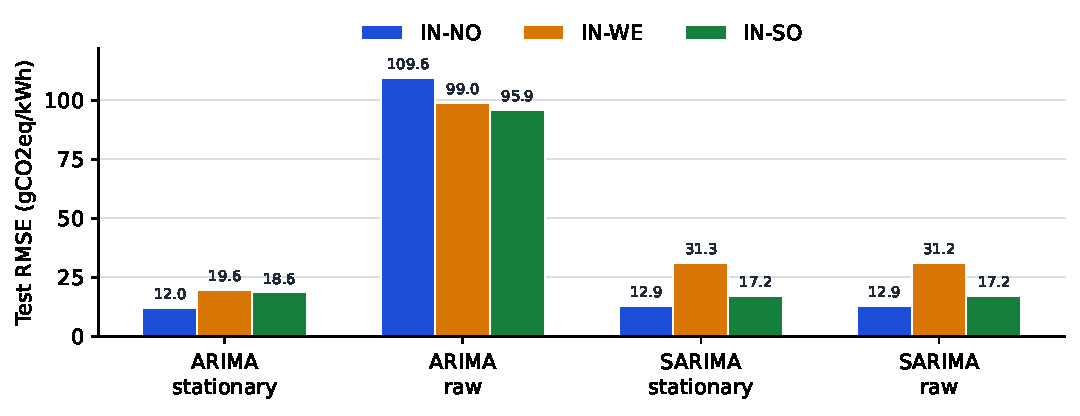
\includegraphics[width=0.94\linewidth]{figures/model_rmse_comparison.pdf}
\caption{RMSE on the same unseen 168-hour test period. Lower is better.}
\end{figure}

\begin{table}[h]
\centering
\small
\rowcolors{2}{lightgray}{white}
\begin{tabular}{lrrrr}
\toprule
Region & ARIMA stat. & ARIMA raw & SARIMA stat. & SARIMA raw \\
\midrule
IN-NO & \textbf{11.96} & 109.60 & 12.94 & 12.92 \\
IN-WE & \textbf{19.61} & 99.03 & 31.28 & 31.24 \\
IN-SO & 18.60 & 95.89 & \textbf{17.21} & 17.24 \\
\bottomrule
\end{tabular}
\caption{Test RMSE in gCO$_2$eq/kWh for the four required models.}
\end{table}

\textbf{Interpretation.} Raw ARIMA performs poorly because ordinary first differencing does not represent the dominant 24-hour structure well. Stationary ARIMA is strongest in IN-NO and IN-WE. Stationary SARIMA is strongest in IN-SO, where explicit seasonal dependence adds useful information.

\newpage

\section{Why SARIMA Is the Strongest General Framework}

SARIMA is the best structural starting point for this problem because the signal is seasonal by design, not by accident. Electricity demand, solar output and operating schedules repeat each day. SARIMA represents this directly through a seasonal period of 24 hours and separate seasonal AR and MA terms.

Three findings support this choice:

\begin{enumerate}
  \item the ACF has strong peaks at daily lags;
  \item lag-24 differencing improves stationarity in every region; and
  \item IN-SO obtains its lowest error from stationary SARIMA.
\end{enumerate}

However, SARIMA is a framework rather than an automatic winner. The final week shows that a simpler stationary ARIMA is more accurate in IN-NO and IN-WE. Therefore, the practical rule is: begin with seasonal reasoning, compare against simpler models and select region-specific parameters using held-out error. This avoids claiming that extra complexity is always useful.

\section{Review 2: Forecast Implementation}

Review 2 converted the Review 1 findings into a fair forecasting experiment.

\begin{itemize}
  \item \textbf{Chronological design:} the recent modelling window uses 180 training days, 7 validation days and a final untouched 7-day test set. Data is never shuffled.
  \item \textbf{Common horizon:} every model predicts the same 168 future hours.
  \item \textbf{Baselines:} a last-value forecast and a 24-hour seasonal-naive forecast set minimum performance targets.
  \item \textbf{Additional models:} leakage-safe SARIMAX, two Holt-Winters models, Random Forest and an MLP neural network provide wider comparison.
  \item \textbf{SARIMAX control:} the true future renewable percentage is not revealed. A seasonal-naive renewable forecast is supplied instead.
  \item \textbf{Accuracy:} MAE, RMSE, MAPE, sMAPE and $R^2$ are calculated on the original carbon-intensity scale.
  \item \textbf{Residual checks:} mean error, residual spread, Jarque-Bera and lag-24 Ljung-Box tests identify bias, non-normality and remaining daily structure.
\end{itemize}

\begin{table}[h]
\centering
\small
\begin{tabularx}{\linewidth}{l X r r r}
\toprule
Region & Overall winning model & RMSE & MAE & $R^2$ \\
\midrule
IN-NO & ARIMA stationary on $\Delta_{24}$ & 11.96 & 9.39 & 0.981 \\
IN-WE & ARIMA stationary on $\Delta_{24}$ & 19.61 & 16.16 & 0.934 \\
IN-SO & SARIMA stationary on $\Delta_{24}$ & 17.21 & 13.71 & 0.956 \\
\bottomrule
\end{tabularx}
\caption{Best model in each region on the shared final week.}
\end{table}

All three winners beat the seasonal-naive baseline. Their residuals still contain significant lag-24 dependence, so the forecasts are useful but not perfect. A production system should retrain often, use rolling-origin validation and publish prediction intervals.

\newpage

\section{Regional Work and Individual Contribution}

The team used one shared method so that results could be compared directly, while each member owned a regional study.

\begin{table}[h]
\centering
\small
\begin{tabularx}{\linewidth}{p{0.12\linewidth} p{0.22\linewidth} X}
\toprule
Region & Contributor & Individual approach and contribution \\
\midrule
IN-NO & Tejeshwar C D R & Prepared the Northern dataset and notebook; completed trend, stationarity and dependence analysis; implemented the common forecast suite; interpreted the strong result from stationary ARIMA. \\
IN-SO & Shantharam P & Completed the Southern regional analysis; examined its renewable-heavy daily behaviour; compared the four required models; documented why stationary SARIMA gives the best Southern forecast. \\
IN-WE & Harish Krishna B & Completed the Western regional analysis; prepared the long hourly history; compared statistical, smoothing and learned models; interpreted the Western result and its larger forecast error. \\
\bottomrule
\end{tabularx}
\caption{Regional ownership and evidence in the final notebooks.}
\end{table}

\section{Cross-Region Interpretation}

The full-period average carbon intensity is approximately 554 for IN-NO, 548 for IN-SO and 671 gCO$_2$eq/kWh for IN-WE. Renewable share and carbon intensity have a strong negative relationship in every region. Their cleanest hours do not occur at exactly the same time. This diversity creates an opportunity to route flexible demand across both time and geography, subject to capacity, cost, latency, reliability and data-residency limits.

\section{Conclusion}

Grid Pulse shows that data preparation and seasonal reasoning matter more than model complexity alone. The raw series changes over time and repeats every 24 hours. Lag-24 differencing creates a more stable forecasting input and produces the best required model in every region. SARIMA is the strongest general framework because it matches the physical daily cycle, and it is the best measured choice for IN-SO. Stationary ARIMA remains more accurate for IN-NO and IN-WE during the shared test week, so final deployment should remain region-specific.

The project meets its main intention: it provides a transparent and reproducible way to understand regional carbon intensity, compare forecasts fairly and support cleaner scheduling decisions.

\section{Data, Code and References}

\textbf{Dataset download:} \href{https://github.com/Shan713/grid-pulse/archive/refs/heads/main.zip}{Download the complete Grid Pulse repository and CSV datasets}. Individual regional files and executed notebooks are available at \href{https://github.com/Shan713/grid-pulse}{github.com/Shan713/grid-pulse}.

\small
\begin{enumerate}
  \item Electricity Maps, ``API documentation,'' \url{https://portal.electricitymaps.com/docs/getting-started}.
  \item statsmodels, ``Time Series Analysis,'' \url{https://www.statsmodels.org/stable/tsa.html}.
  \item scikit-learn, ``User Guide,'' \url{https://scikit-learn.org/stable/user_guide.html}.
\end{enumerate}

\end{document}
